%% 
%% Copyright 2007-2018 Elsevier Ltd
%% 
%% This file is part of the 'Elsarticle Bundle'.
%% ---------------------------------------------
%% 
%% It may be distributed under the conditions of the LaTeX Project Public
%% License, either version 1.2 of this license or (at your option) any
%% later version.  The latest version of this license is in
%%    http://www.latex-project.org/lppl.txt
%% and version 1.2 or later is part of all distributions of LaTeX
%% version 1999/12/01 or later.
%% 
%% The list of all files belonging to the 'Elsarticle Bundle' is
%% given in the file `manifest.txt'.
%% 

%% Template article for Elsevier's document class `elsarticle'
%% with numbered style bibliographic references
%% SP 2008/03/01
%%
%% 
%%
%% $Id: elsarticle-template-num.tex 64 2013-05-15 12:23:51Z rishi $
%%
%%
\documentclass[preprint,12pt,3p]{elsarticle}

%% Use the option review to obtain double line spacing
%% \documentclass[authoryear,preprint,review,12pt]{elsarticle}

%% Use the options 1p,twocolumn; 3p; 3p,twocolumn; 5p; or 5p,twocolumn
%% for a journal layout:
%% \documentclass[final,1p,times]{elsarticle}
%% \documentclass[final,1p,times,twocolumn]{elsarticle}
%% \documentclass[final,3p,times]{elsarticle}
%% \documentclass[final,3p,times,twocolumn]{elsarticle}
%% \documentclass[final,5p,times]{elsarticle}
%% \documentclass[final,5p,times,twocolumn]{elsarticle}

%% For including figures, graphicx.sty has been loaded in
%% elsarticle.cls. If you prefer to use the old commands
%% please give \usepackage{epsfig}

%% The amssymb package provides various useful mathematical symbols
\usepackage{amssymb}
\usepackage{textcomp}
\usepackage[version=4]{mhchem}
%% The amsthm package provides extended theorem environments
%% \usepackage{amsthm}

%% The lineno packages adds line numbers. Start line numbering with
%% \begin{linenumbers}, end it with \end{linenumbers}. Or switch it on
%% for the whole article with \linenumbers.
%% \usepackage{lineno}

\journal{International Journal of Hydrogen Energy}

\begin{document}

\begin{frontmatter}

%% Title, authors and addresses

%% use the tnoteref command within \title for footnotes;
%% use the tnotetext command for theassociated footnote;
%% use the fnref command within \author or \address for footnotes;
%% use the fntext command for theassociated footnote;
%% use the corref command within \author for corresponding author footnotes;
%% use the cortext command for theassociated footnote;
%% use the ead command for the email address,
%% and the form \ead[url] for the home page:
%% \title{Title\tnoteref{label1}}
%% \tnotetext[label1]{}
%% \author{Name\corref{cor1}\fnref{label2}}
%% \ead{email address}
%% \ead[url]{home page}
%% \fntext[label2]{}
%% \cortext[cor1]{}
%% \address{Address\fnref{label3}}
%% \fntext[label3]{}

\title{Hydrogen Production From Aluminum-Water Reactions Subject to High
  Pressures and Temperatures}

%% use optional labels to link authors explicitly to addresses:
%% \author[label1,label2]{}
%% \address[label1]{}
%% \address[label2]{}

\author{Peter Godart}
\author{Jason Fischman}
\author{Kelsey Seto}
\author{Douglas Hart}

\address{Massachusetts Institute of Technology\\77 Massachusetts Avenue, Rm
  3-252\\Cambridge, MA 02139}

\begin{abstract}
%% Text of abstract
Here's some stuff about what we did, blah blah

\end{abstract}

\begin{keyword}
%% keywords here, in the form: keyword \sep keyword
hydrogen production \sep aluminum activation \sep aluminum-water reaction \sep
gibbs free energy \sep reaction favorability \sep byproduct determination

%% PACS codes here, in the form: \PACS code \sep code

%% MSC codes here, in the form: \MSC code \sep code
%% or \MSC[2008] code \sep code (2000 is the default)

\end{keyword}

\end{frontmatter}

%% \linenumbers

%% main text
\section{Introduction}
\label{introduction}

Aluminum is a great fuel, etc.

\section{Model}
\label{model}

In order to predict the reaction products of an aluminum water reaction over a
wide range of temperatures and pressures, we use the Gibbs free energy to
determine which reaction is most favorable at given ambient conditions. To
perform this analysis, it was first necessary to determine which reactions could
possibly be occurring, and since aluminum, hydrogen, and oxygen can form a wide
variety of compounds, it was also desirable to narrow down this list.

Simple experiments that measure the output of hydrogen from an aluminum water
reaction at atmospheric pressure and 20 \textdegree C conditions as in [Cite
jonny?] have shown that 3 moles of hydrogen are generated for every 2 moles of
aluminum reacted (do we want to include this experiment in this paper? easy to
show Jason reaction completion data? can plot hydrogen yield as molar ratio to
input aluminum). Consequently, the reaction that occurs can be one of the
following:

Using a setup shown in Figure XX, we measured the hydrogen evolved from the
reaction of aluminum and water at 1 bar and 20 \textdegree C. From this simple
experiment, we determined that roughly 3 moles of hydrogen were produced for
every two moles of aluminum (do we need to talk about assuming the reaction
proceeded to completion here? We determined from byproducts that no elemental
aluminum was left in the reaction products?)...

Consequently, we determined that the most likely reactions to occur are the
ones in which yield hydrogen in a stoichiometric ratio of 3:2 with aluminum.
These reactions are

\begin{equation}
  \ce{2Al_{(s)} + 6H2O_{(l)} -> 3H2_{(g)} + 2Al(OH)3_{(aq)} + Q}
  \label{eq:hydroxide}
\end{equation}

\begin{equation}
  \ce{2Al_{(s)} + 4H2O_{(l)} -> 3H2_{(g)} + 2AlOOH_{(aq)} + Q}
  \label{eq:oxyhydroxide}
\end{equation}

\begin{equation}
  \ce{2Al_{(s)} + 2H2O_{(l)} -> 3H2_{(g)} + 2Al2O3_{(aq)} + Q.}
  \label{eq:oxide}
\end{equation}

For each of these reactions, we compute the change in Gibbs free energy,
$\Delta_fG(T,p)$, between the products and reactants. For example, the change in
Gibbs free energy for reaction \ref{eq:hydroxide} would be given by

\begin{equation}
  \Delta_fG^{(1)} = (2\cdot g_{Al(OH)_3} + 3\cdot g_{H_2}) - (2\cdot g_{Al} + 6\cdot g_{H_2O}),
\end{equation}

\noindent where $g_{Al(OH)_3}$, for example, is the Gibbs free energy of
aluminum hydroxide, $Al(OH)_3$ at a given temperature and pressure.

The sign and magnitude of this quantity indicate whether the reaction in
question can occur spontaneously without outside influence and its relative
favorability over other possible reactions. Specifically, for $\Delta_fG(T,p) <
0$, the reaction is spontaneous and for $\Delta_fG(T,p) > 0$, the reaction will
not occur with outside influence. A reaction without a change in Gibbs free
energy ($\Delta_fG(T,p) = 0$) is in equilibrium. When multiple reactions are
possible, the most favorable reaction is the one that minimizes the Gibbs free
energy at a particular temperature and pressure.

Literature values for the Gibbs free energy of the species involved in these
reaction are given for a wide range of temperatures as shown in [] and [] but
only for 1 bar. Our goal, however, is to model the aluminum water reaction over
a range of operating pressures as well. As shown in Appendix A, the change in
Gibbs free energy for a species at non-atmospheric temperature and pressures is
given as

\begin{equation}
  \Delta_f g(T,p) = \Delta_f g^{0}(T) + v(p-p_0)
  \label{eq:gibbs_solid}
\end{equation}

\noindent for solid, liquid, or aqueous species and

\begin{equation}
  \Delta_f g(T,p) = \Delta_f g^{0}(T) + RT\ln\left(\frac{p}{p_0}\right) 
  \label{eq:gibbs_gas}
\end{equation}

\noindent for gaseous species. In both cases $\Delta_f g^0$ is the change in
Gibbs free energy per mole of species $i$ at 1 bar and is given in literature,
$v$ is the specific volume of species $i$, and R is the ideal gas constant. It
is important to note that in Equation \ref{eq:gibbs_gas}, $p$ is the partial
pressure of the gas species, whereas $p$ in Equation \ref{eq:gibbs_solid} is the
total ambient pressure. To compute the change in Gibbs free energy for each of
the candidate aluminum water reactions, we apply the stoichiometric ratios in
Equations \ref{eq:hydroxide}-\ref{eq:oxide} to the appropriate expression for
molar change in Gibbs free energy, depending on the phase of each species.

For this analysis, we neglect the presence of air or other inert gases as well
as the formation of steam that could occur due to the exothermic nature of
aluminum water reactions. To be completely accurate, these must be accounted for
as well, but because their presence is highly dependent on reaction
configurations, it is difficult to generalize their influence. The presence of
other inert gases is typically negligible as the partial pressure of hydrogen
reaction product appears inside a natural logarithm term in Equation
\ref{eq:gibbs_gas}. The formation of steam, however, would be significant and
should be the focus of future work.

To determine which reaction is most favorable at a given constant temperature
and pressure, we seek the reaction that minimizes $\Delta_f G(T,p)$. Using
values for $g_i^0(T)$ given by [NASA] and [oxyhydroxide paper] for $AlOOH$, we
computed Gibbs free energy surfaces for each of the three candidate aluminum
water reactions, as shown in Figure \ref{fig:gibbs_surface}. At a given
temperature and pressure, the most negative Gibbs free energy surface at that
point will be the most favorable reaction to occur. To highlight where these
transitions occur, we can project the minimum surface values onto the $T$-$p$
plane, as shown in Figure \ref{fig:transitions_full}, clearly showing which reaction
is favorable for each $(T,p)$.

\begin{figure}
  \centering
  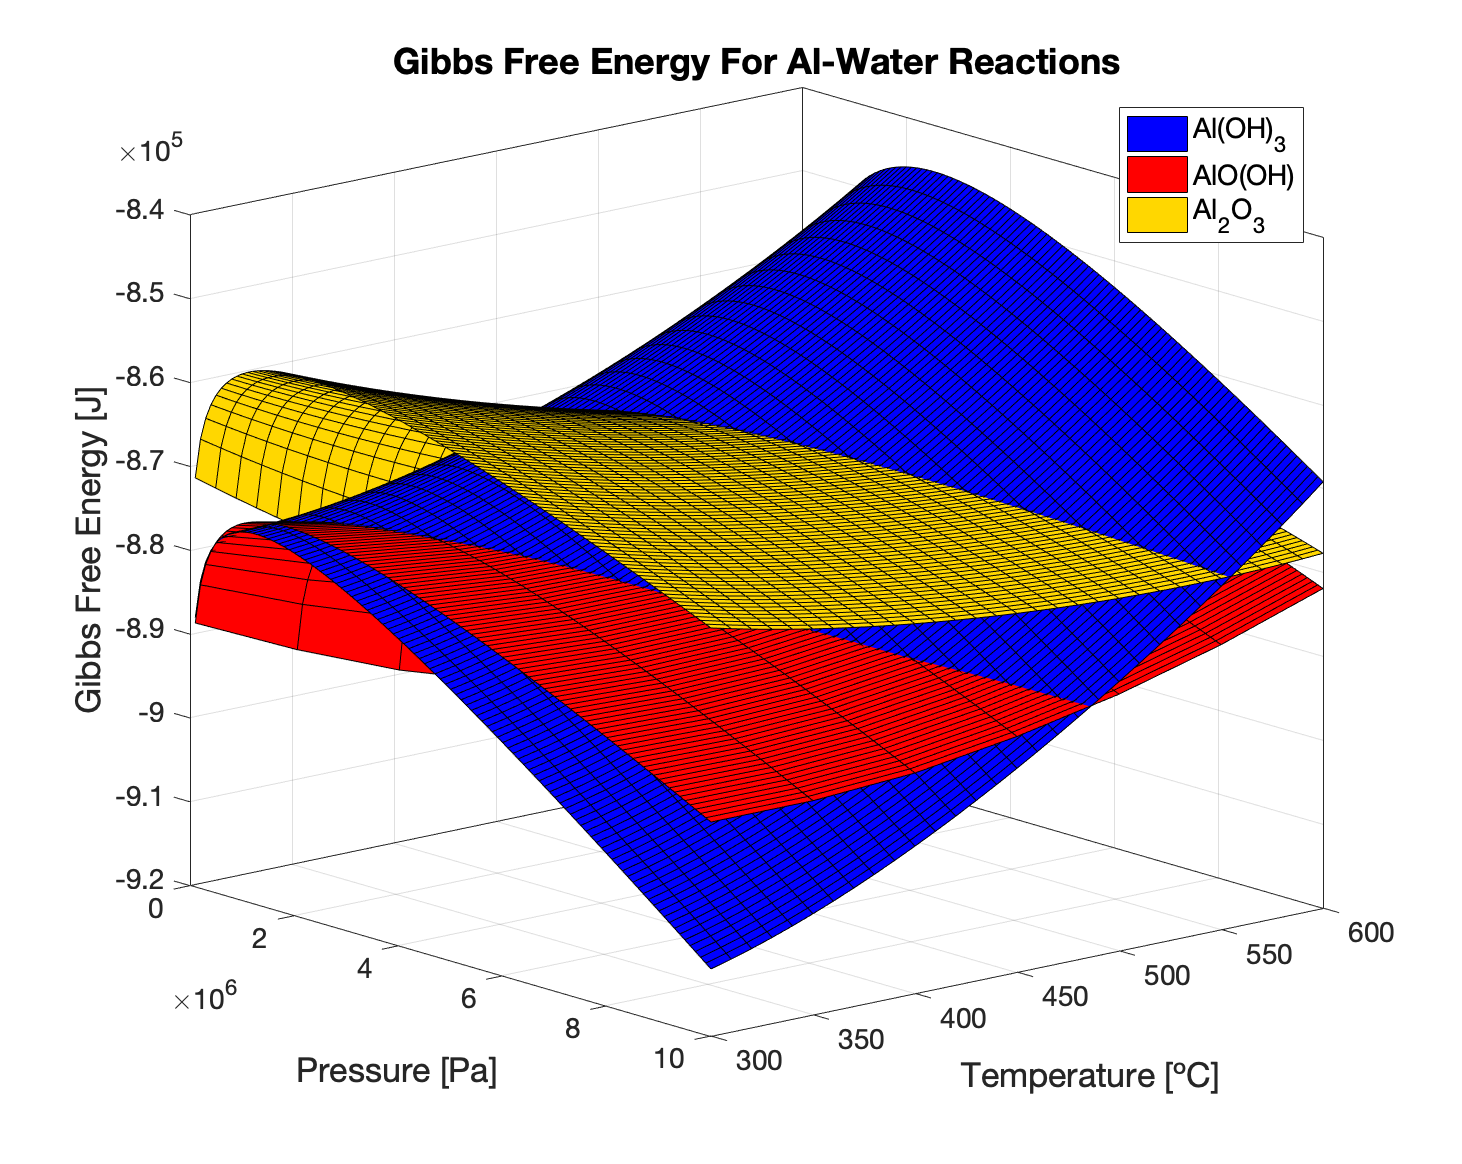
\includegraphics[width=0.8\textwidth]{fig/gibbs_total_surface}
  \label{fig:gibbs_surface}
\end{figure}

\begin{figure}
  \centering
  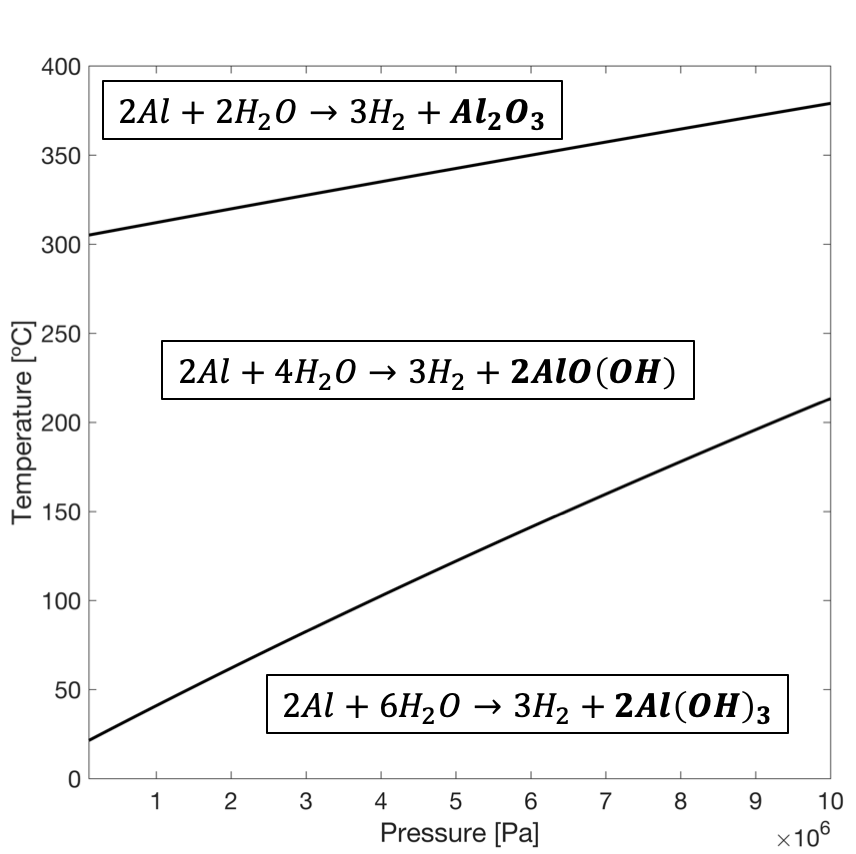
\includegraphics[width=0.7\textwidth]{fig/transitions}
  \label{fig:transitions_full}
\end{figure}

\subsection{Limited Reactivity with Steam}

We have also shown that steam does not react with...

\section{Materials}
\label{materials}

\subsection{Aluminum Activation}

\section{Experimental}
\label{experiment}

\section{Results}
\label{results}

\section{Discussion}
\label{discussion}

\section{Conclusion}
\label{conclusion}

%% The Appendices part is started with the command \appendix;
%% appendix sections are then done as normal sections
%% \appendix

%% \section{}
%% \label{}

%% If you have bibdatabase file and want bibtex to generate the
%% bibitems, please use
%%
%%  \bibliographystyle{elsarticle-num} 
%%  \bibliography{<your bibdatabase>}

%% else use the following coding to input the bibitems directly in the
%% TeX file.

\begin{thebibliography}{00}

%% \bibitem{label}
%% Text of bibliographic item

\bibitem{}

\end{thebibliography}
\end{document}
\endinput
%%
%% End of file `elsarticle-template-num.tex'.
